\documentclass[10pt]{beamer}
\usefonttheme{professionalfonts}
%\usetheme{CambridgeUS}
%
% Choose how your presentation looks.
%
% For more themes, color themes and font themes, see:
% http://deic.uab.es/~iblanes/beamer_gallery/index_by_theme.html
%
\mode<presentation>
{
  \usetheme{default}      % or try Darmstadt, Madrid, Warsaw, ...
  \usecolortheme{beaver} % or try albatross, beaver, crane, ...
  \usefonttheme{default}  % or try serif, structurebold, ...
  \setbeamertemplate{navigation symbols}{}
  \setbeamertemplate{caption}[numbered]
} 

\usepackage[english]{babel}
\usepackage[utf8x]{inputenc}
\usepackage{tikz}
\usepackage{pgfplots}
\usepackage{array}  % for table column M
\usepackage{makecell} % to break line within a cell
\usepackage{verbatim}
\usepackage{graphicx}
\usepackage{subcaption}
\usepackage{amsfonts}
\usepackage{amsmath}
\usepackage{bm}
\usepackage{epstopdf}
\captionsetup{compatibility=false}
%\usepackage{dsfont}
\usepackage[absolute,overlay]{textpos}
\usetikzlibrary{calc}
\usetikzlibrary{pgfplots.fillbetween, backgrounds}
\usetikzlibrary{positioning}

\usetikzlibrary{pgfplots.groupplots}
\usetikzlibrary{plotmarks}
\usetikzlibrary{calc}

\usepgfplotslibrary{groupplots}
\pgfplotsset{compat=newest} 
%\pgfplotsset{plot coordinates/math parser=false}

\usepackage{hyperref}
\hypersetup{
    colorlinks=true,
    linkcolor=blue,
    filecolor=magenta,      
    urlcolor=cyan,
}

%% 
%\def\EXTERNALIZE{1} % for externalizing figures
\input{header.tex}

\DeclareRobustCommand\sampleline[1]{%
	\tikz\draw[#1] (0,0) (0,\the\dimexpr\fontdimen22\textfont2\relax)
	-- (2em,\the\dimexpr\fontdimen22\textfont2\relax);%
}

%%
\title[The Hebbian-LMS Algorithm]{Hebbian Learning and the LMS Algorithm}
\author{Prof. Bernard Widrow \\ Jose Krause Perin \\ Hakim Mesiwala \\ Youngsik Kim \\ Dookun Park}
\institute{\normalsize Department of Electrical Engineering \\ Stanford University}
\date{IEEE SCV \textbullet~September 26, 2017}

\begin{document}

\begin{frame}
  \titlepage
\end{frame}

\begin{frame}{Adaptive linear neuron (Adaline)}
\begin{center}
	\includegraphics[page=2,width=0.95\textwidth, trim={2cm 1.75cm 2cm 1.5cm}, clip]{figures.pdf}
\end{center}
\end{frame}

\begin{frame}{Knobby Adaline, 1959}
\begin{center}
	\includegraphics[page=3,width=0.95\textwidth, trim={2cm 2.5cm 2cm 1.5cm}, clip]{figures.pdf}
\end{center}
\end{frame}

\begin{frame}{Bootstrap learning}
\begin{center}
	\includegraphics[page=4,width=0.95\textwidth, trim={0.5cm 3.9cm 0.5cm 1.5cm}, clip]{figures.pdf}
\end{center}
\end{frame}

\begin{frame}{Bootstrap learning}
\begin{center}
	\includegraphics[page=5,width=0.95\textwidth, trim={0.5cm 2.5cm 0.5cm 1.5cm}, clip]{figures.pdf}
\end{center}
\end{frame}

\begin{frame}{Bootstrap learning}
\begin{center}
	\includegraphics[page=6,width=0.95\textwidth, trim={0.5cm 2.5cm 0.5cm 1.5cm}, clip]{figures.pdf}
\end{center}
\end{frame}

\begin{frame}{Decision-directed learning for channel equalization}
\begin{center}
	\includegraphics[page=7,width=0.95\textwidth, trim={1cm 0.75cm 1cm 1.5cm}, clip]{figures.pdf}
\end{center}
\end{frame}

\begin{frame}{Eye diagrams}
\begin{center}
	\includegraphics[page=8,width=\textwidth, trim={0.4cm 4.5cm 0.4cm 1.5cm}, clip]{figures.pdf}
\end{center}
\end{frame}

\begin{frame}{Training neurons with bootstrap learning}
\begin{center}
	\resizebox{\textwidth}{!}{\def\layersep{0.5cm}
\def\outsep{0.7cm}
\def\dy{0.5}

\begin{tikzpicture}[>=stealth, shorten >= 0pt, draw=black!50, node distance=\layersep, font=\sffamily]
    \tikzstyle{node}=[circle,fill=black,minimum size=2pt,inner sep=0pt]
    \tikzstyle{weight}=[draw=black,circle,fill=none,minimum size=3pt,inner sep=0pt,scale=0.5]
    \tikzstyle{summer}=[weight,scale=1.8, minimum size=15pt]
    \tikzstyle{sigmoid}=[draw=black,rectangle,fill=none,minimum size=20pt,inner sep=0pt]
    \tikzstyle{annot} = [scale=0.5]

	\node[summer] (Adder) at (3*\layersep,-\dy*2.5 cm) {\large $\Sigma$}; 
    \node[node, inner sep=0pt] (mid) at (4.5*\layersep,-\dy*2.5 cm) {}; 
    \node[sigmoid] (SGM) at (6*\layersep,-\dy*2.5 cm) {\resizebox{18pt}{!}{\begin{tikzpicture} 
\begin{axis}[
axis lines*=middle,
enlargelimits = true,
xmax=6,
xmin=-6,
ymin=-1,
ymax=1,
xtick=\empty,
ytick=\empty,
  ]
\addplot[black, line width=2pt, domain=-6:6, samples=50] {-1+2/(1+exp(-x))};
\end{axis}
\end{tikzpicture}
}}; % Draw the hidden layer 
    \node[node, inner sep=0pt] (output-tap) at (7.3*\layersep,-\dy*2.5 cm) {};
    \coordinate (output) at (8*\layersep,-\dy*2.5 cm) {};
    \node[summer, minimum size=10pt, scale=1] (error) at (6*\layersep,-\dy*5 cm) {$\Sigma$}; 
    \coordinate (xw) at (4.5*\layersep,-\dy*5 cm) {};
    \coordinate (out) at (7.3*\layersep,-\dy*5 cm) {};
    \node[weight,fill=white, scale=1.5] (gamma) at (4.5*\layersep,-\dy*4 cm) {$\gamma$};
    \coordinate (error-out) at (6*\layersep,-\dy*6 cm) {};
    
    \coordinate (A) at (\layersep,-6*\dy cm) {};
    \coordinate (B) at (\layersep,\dy cm) {};
    \path[->] (A) edge (B);
    \path[-] (error) edge (error-out);
    \path[-] (error-out) edge (A);
        
    \foreach \name / \y in {0,...,3} {
    % This is the same as writing \foreach \name / \y in {1/1,2/2,3/3,4/4}
        \node[node] (I-\name) at (0,-\dy*\y) {}; % Draw the input layer nodes
        \node[weight,fill=white] (W-\name) at (\layersep,-\dy*\y cm) {$W_{k\name}$}; % Draw the hidden layer  layer node     
     }   	

	\node[node] (I-4) at (0,-5*\dy cm) {}; % Draw the hidden layer 
	\node[weight, fill=white] (W-4) at (\layersep,-5*\dy cm) {$W_{kn}$};
	
    %% Annotations
    \node[scale=0.5] at (-0.3,0) {$+1$};
    \node[scale=0.5] at (-0.3,-\dy) {$X_{k1}$};
    \node[scale=0.5] at (-0.3,-\dy*2) {$X_{k2}$};
    \node[scale=0.5] at (-0.3,-\dy*3) {$X_{k3}$};
    \node[scale=0.5] at (-0.3,-\dy*5) {$X_{kn}$};
    \node[scale=0.5] at (-0.3,-\dy*3.75) {$\vdots$};
    
    \node[font=\fontsize{3}{3}\selectfont] at (6*\layersep-7,-\dy*4.7 cm) {$-$};
    \node[font=\fontsize{3}{3}\selectfont] at (6*\layersep+7,-\dy*4.7 cm) {$+$};
    \node[annot] at (3*\layersep+7,-\dy*5.7 cm) {error $\epsilon_k$};
    \node[annot] at (4.3*\layersep,-\dy*2 cm) {$(X_k^TW_k)$};
    \node[annot] at (8.7*\layersep,-\dy*2.5 cm) {Output};
    \node[annot] at (6*\layersep,-\dy*3.5 cm) {Sigmoid};
    
    \foreach \name in {0,...,4} {
    		\path[->] (I-\name) edge (W-\name);
            \path[->] (W-\name) edge (Adder);
     }
	
    \path[-] (Adder) edge (mid);
    \path[->] (mid) edge (SGM);
    \path[->] (mid) edge (gamma);
    \path[-] (gamma) edge (xw);
    \path[->] (xw) edge (error);
    \path[-] (SGM) edge (output-tap);
    \path[->] (output-tap) edge (output);
    \path[-] (output-tap) edge (out);
    \path[->] (out) edge (error);
    
    \draw[-,decoration={brace,mirror,raise=5pt},decorate, thick]
   (-0.35,-0.7*\dy) -- node[annot, left=5pt, text width = 1cm, align=center] {$X_k$ input} (-0.35,-\dy*5.2);
   
   \node[draw=black, inner sep=5pt, fill=blue2!20, above=0.5cm of SGM, text width=5cm, align=left, scale=0.6] (eq1) {Hebbian-LMS algorithm  \begin{equation*}
   	\begin{cases}
   	W_{k+1} = W_k + 2\mu\epsilon_kX_k \\ 
   	\epsilon_k = \mathrm{SGM}(X_k^TW_k) - \gamma(X_k^TW_k)
   	\end{cases}
   	\end{equation*}
   };
\end{tikzpicture}}
\end{center}
\end{frame}

\begin{frame}{Equilibrium points of Hebbian-LMS}
\begin{center}
	\resizebox{0.95\textwidth}{!}{%%% START MACRO %%%
\newcommand{\slopeTriangle}[5]
{
    % #1. Relative offset in x direction.
    % #2. Width in x direction, so xA-xB.
    % #3. Relative offset in y direction.
    % #4. Slope dydx.
    % #5. Plot options.

    \pgfplotsextra
    {
        \pgfkeysgetvalue{/pgfplots/xmin}{\xmin}
        \pgfkeysgetvalue{/pgfplots/xmax}{\xmax}
        \pgfkeysgetvalue{/pgfplots/ymin}{\ymin}
        \pgfkeysgetvalue{/pgfplots/ymax}{\ymax} 

        % Calculate auxilliary quantities.
        \pgfmathsetmacro{\xA}{\xmin+(#1+#2)*(\xmax-\xmin)}
        \pgfmathsetmacro{\yA}{\ymin+#3*(\ymax-\ymin)}
        \pgfmathsetmacro{\xB}{\xmin+#1*(\xmax-\xmin)}
        \pgfmathsetmacro{\yB}{\yA}
        \pgfmathsetmacro{\xC}{\xA}
        \pgfmathsetmacro{\yC}{\yA+(\xA-\xB)*#4}

        % Define coordinates for \draw.
        \coordinate (A) at (axis cs:\xA,\yA);
        \coordinate (B) at (axis cs:\xB,\yB);
        \coordinate (C) at (axis cs:\xC,\yC);

        % Draw slope triangle.
        \draw[#5]   (A)-- node[pos=0.5,anchor=north, scale = 0.7] {1}
                    (B)-- 
                    (C)-- node[pos=0.5, scale=0.7] {$\gamma$}
                    cycle;
    }
}
%%% END MACRO %%%

\tikzset{
  double arrow/.style args={#1 colored by #2 and #3}{
    >=stealth, ultra thick, ->,line width=(#1)/3,#2, % first arrow
    postaction={draw,>=stealth, ultra thick, ->,#3,line width=(#1)/5,
                shorten <=(#1)/5,shorten >=2*(#1)/5}, % second arrow
  }
}

\def\intersect{9.999}
\begin{tikzpicture} 
\begin{axis}[
axis lines*=middle,
enlargelimits = true,
xmax=15,
xmin=-15,
ymin=-1.5,
ymax=1.5,
axis line style={->},
xlabel style={text width = 0.5cm, scale=0.7}, xlabel={\small $(X^TW)$},
ylabel style={text width = 0.5cm, scale=0.7}, ylabel={\small Sigmoid Output},
every axis x label/.style={
    at={(ticklabel* cs:1)},
    anchor=north,
},
every axis y label/.style={
    at={(ticklabel* cs:1)},
    anchor=south,
},
xtick=\empty,
ytick={-1, 1},
yticklabels={$-1$, $1$},
yticklabel style={xshift=0.1cm},
xtick={-\intersect, \intersect},
xticklabel=\empty,
%xmajorgrids,
%ymajorgrids,
every outer y axis line/.append style={white!15!black},
every y tick label/.append style={font=\color{white!15!black}},
legend style={draw=white!15!black,fill=white,legend cell align=left}]
\addplot[name path = A, black, line width=1.5pt, domain=-17:17, samples=100] {-1+2/(1+exp(-x))};
\addplot[name path = B, black, line width=1pt, domain=-17:17, samples=2] {0.1*x};


\addplot[blue2!80] fill between[of=A and B, soft clip={domain=0:\intersect}];
\addplot[blue2!80] fill between[of=A and B, soft clip={domain=-17:-\intersect}];
\addplot[Qred!80] fill between[of=A and B, soft clip={domain=-\intersect:0}];
\addplot[Qred!80] fill between[of=A and B, soft clip={domain=\intersect:17}];


\node[draw,circle,minimum width = 0.3cm,inner sep=0pt, fill=white] at (4,0.7) {\textbf{$+$}};
\node[draw,circle,minimum width = 0.3cm,inner sep=0pt, fill=white] at (-15,-1.25) {\textbf{$+$}};
\node[draw,circle,minimum width = 0.3cm,inner sep=0pt, fill=white] at (-4,-0.7) {\textbf{$-$}};
\node[draw,circle,minimum width = 0.3cm,inner sep=0pt, fill=white] at (15,1.25) {\textbf{$-$}};

\node[coordinate,pin={[pin edge={solid, semithick}, align=center, scale=0.6, text width = 2.5cm, pin distance=0.5cm]-85:{Stable equilibrium point}}] at (axis cs:\intersect,1){};
\node[coordinate,pin={[pin edge={solid, semithick}, align=center, scale=0.6, text width = 2.5cm]-75:{Unstable equilibrium point}}] at (axis cs:0,0){};
\node[coordinate,pin={[pin edge={solid, semithick}, align=center, scale=0.6, text width = 2.5cm]95:{Stable equilibrium point}}] at (axis cs:-\intersect,-1){};
\node[coordinate,pin={[pin edge={solid, semithick}, align=center, scale=0.6]105:{slope $\gamma$}}] at (axis cs:14,1.4){};
\node[coordinate,pin={[pin edge={solid, semithick}, align=center, scale=0.6]-75:{slope $\gamma$}}] at (axis cs:-14,-1.4){};

%\draw[double arrow = 7pt colored by white and blue2!120] (axis cs:7,0.85) -- (axis cs:9, 0.97);
%\draw[white, line width = 0.9mm, ->, >=stealth] (axis cs:7,0.85) -- (axis cs:9, 0.97);
\draw[blue2!20, line width = 0.6mm, ->, >=stealth, shorten <=1pt,shorten >=1pt] (axis cs:7,0.85) -- (axis cs:9, 0.97);

%\draw[white, line width = 0.9mm, ->, >=stealth] (axis cs:13, 1.15) -- (axis cs:11,1.03);
\draw[Qred!20, line width = 0.6mm, ->, >=stealth, shorten <=1pt,shorten >=1pt] (axis cs:13, 1.15) -- (axis cs:11,1.03);

%\draw[white, line width = 0.9mm, ->, >=stealth] (axis cs:-7,-0.85) -- (axis cs:-9, -0.97);
\draw[Qred!20, line width = 0.6mm, ->, >=stealth, shorten <=1pt,shorten >=1pt] (axis cs:-7,-0.85) -- (axis cs:-9, -0.97);

%\draw[white, line width = 0.9mm, ->, >=stealth] (axis cs:-13, -1.15) -- (axis cs:-11,-1.03);
\draw[blue2!20, line width = 0.6mm, ->, >=stealth, shorten <=1pt,shorten >=1pt] (axis cs:-13, -1.15) -- (axis cs:-11,-1.03);

%\slopeTriangle{0.57}{0.07}{0.573}{0.1}{black}; % USE OF MACRO.

\end{axis}
\end{tikzpicture}
}
\end{center}
\end{frame}

\begin{frame}{Hebbian-LMS learning process}
\large Random initial weights: some input patterns produce {\color{green2} \textbf{positive output}}, while others produce {\color{orange2} \textbf{negative output}}
\begin{center}
	\resizebox{0.85\textwidth}{!}{\begin{tikzpicture}
\begin{axis}[
axis lines*=middle,
enlargelimits = true,
axis line style={->},
xlabel style={text width = 0.5cm, scale=0.7}, xlabel={\small $(X^TW)$},
ylabel style={text width = 0.5cm, scale=0.7}, ylabel={\small Sigmoid Output},
every axis x label/.style={
    at={(ticklabel* cs:1)},
    anchor=north,
},
every axis y label/.style={
    at={(ticklabel* cs:1)},
    anchor=south,
},
xtick=\empty,
ytick=\empty,
xticklabel=\empty,
yticklabel=\empty,
xmax=5,
xmin=-5,
ymax=1.2,
ymin=-1.2,
every outer y axis line/.append style={white!15!black},
every y tick label/.append style={font=\color{white!15!black}},
legend style={draw=white!15!black,fill=white,legend cell align=left}]
\addplot[gray, name path = A, black, line width=1pt, domain=-6:6, samples=50] {(1 - exp(-2*x))/(1 + exp(-2*x))};
\addplot[gray, name path = A, black, line width=0.5pt, domain=-6:6, samples=2] {0.3*x};

\addplot [color=green2, only marks, mark=star, line width = 1.5pt, mark size=4pt, forget plot]
table[row sep=crcr]{
	1.2049 0.83514 \\
	6.3427 0.99999 \\
	9.5248 1 \\
	1.9315 0.95886 \\
	4.1213 0.99947 \\
	5.2604 0.99995 \\
	3.1462 0.99631 \\
	2.9045 0.99402 \\
	5.4438 0.99996 \\
	3.9238 0.99922 \\
	1.2255 0.84126 \\
	6.1231 0.99999 \\
	0.41799 0.39523 \\
	4.5207 0.99976 \\
	1.5911 0.92033 \\
	2.0125 0.9649 \\
	1.2447 0.8468 \\
	3.7051 0.99879 \\
	5.2149 0.99994 \\
	4.4333 0.99972 \\
	9.2895 1 \\
	1.8718 0.95376 \\
	3.8262 0.99905 \\
	3.3879 0.99772 \\
	4.2188 0.99957 \\
	2.3713 0.98272 \\
	5.6295 0.99997 \\
	11.6232 1 \\
	3.7974 0.99899 \\
	7.6905 1 \\
	0.48676 0.45164 \\
	7.1896 1 \\
	7.0757 1 \\
	4.1376 0.99949 \\
	9.8504 1 \\
	4.2193 0.99957 \\
	7.8673 1 \\
	4.3483 0.99967 \\
	0.82362 0.67704 \\
	9.2187 1 \\
	0.52234 0.4795 \\
	2.8783 0.9937 \\
	1.3284 0.86886 \\
	0.1326 0.13183 \\
	7.8745 1 \\
};

\addplot [color=orange2, only marks, mark=star, line width = 1.5pt, mark size=4pt, forget plot]
table[row sep=crcr]{
	-9.9594 -1 \\
	-5.9728 -0.99999 \\
	-0.32759 -0.31635 \\
	-2.1754 -0.97454 \\
	-7.2578 -1 \\
	-6.0416 -0.99999 \\
	-3.5325 -0.99829 \\
	-0.097481 -0.097174 \\
	-3.8781 -0.99914 \\
	-7.2676 -1 \\
	-0.42272 -0.39922 \\
	-5.9569 -0.99999 \\
	-2.9095 -0.99408 \\
	-1.5504 -0.91384 \\
	-4.4754 -0.99974 \\
	-1.2059 -0.83546 \\
	-17.7175 -1 \\
	-3.254 -0.99702 \\
	-5.3958 -0.99996 \\
	-5.0407 -0.99992 \\
	-7.3742 -1 \\
	-2.6891 -0.99081 \\
	-9.2625 -1 \\
	-3.4308 -0.99791 \\
	-1.0805 -0.79338 \\
	-3.3361 -0.99747 \\
	-6.0204 -0.99999 \\
	-3.1419 -0.99627 \\
	-3.3617 -0.9976 \\
	-3.1119 -0.99604 \\
	-1.5888 -0.91997 \\
	-2.2015 -0.97581 \\
	-3.2387 -0.99693 \\
	-2.1778 -0.97465 \\
	-11.6565 -1 \\
	-8.5916 -1 \\
	-15.2291 -1 \\
	-3.0446 -0.99548 \\
	-5.5413 -0.99997 \\
	-11.4804 -1 \\
	-3.8097 -0.99902 \\
	-6.6605 -1 \\
	-9.3825 -1 \\
	-8.9103 -1 \\
	-7.0742 -1 \\
};
\end{axis}
\end{tikzpicture}}
\end{center}
\end{frame}

\begin{frame}{Hebbian-LMS learning process}
\large After 10 training cycles
\begin{center}
	\resizebox{0.85\textwidth}{!}{\begin{tikzpicture}
\begin{axis}[
axis lines*=middle,
enlargelimits = true,
axis line style={->},
xlabel style={text width = 0.5cm, scale=0.7}, xlabel={\small $(X^TW)$},
ylabel style={text width = 0.5cm, scale=0.7}, ylabel={\small Sigmoid Output},
every axis x label/.style={
    at={(ticklabel* cs:1)},
    anchor=north,
},
every axis y label/.style={
    at={(ticklabel* cs:1)},
    anchor=south,
},
xtick=\empty,
ytick=\empty,
xticklabel=\empty,
yticklabel=\empty,
xmax=5,
xmin=-5,
ymax=1.2,
ymin=-1.2,
every outer y axis line/.append style={white!15!black},
every y tick label/.append style={font=\color{white!15!black}},
legend style={draw=white!15!black,fill=white,legend cell align=left}]
\addplot[gray, name path = A, black, line width=1pt, domain=-6:6, samples=50] {(1 - exp(-2*x))/(1 + exp(-2*x))};
\addplot[gray, name path = A, black, line width=0.5pt, domain=-6:6, samples=2] {0.3*x};

\addplot [color=orange2, only marks, mark=star, line width = 1.5pt, mark size=4pt, forget plot]
table[row sep=crcr]{
	-3.6778 -0.99872 \\
	-3.028 -0.99532 \\
	-3.3813 -0.99769 \\
	-2.7108 -0.9912 \\
	-3.8201 -0.99904 \\
	-4.9689 -0.9999 \\
	-2.4537 -0.98533 \\
	-3.8669 -0.99912 \\
	-2.544 -0.98774 \\
	-2.9673 -0.99472 \\
	3.0716 0.99571 \\
	-3.4193 -0.99786 \\
	-0.13987 -0.13896 \\
	0.64482 0.56817 \\
	-2.0753 -0.96898 \\
	1.6772 0.9325 \\
	-4.3642 -0.99968 \\
	-3.2605 -0.99706 \\
	-3.2145 -0.99678 \\
	-2.9369 -0.99439 \\
	-2.1394 -0.97266 \\
	-2.215 -0.97645 \\
	-4.5933 -0.9998 \\
	-2.8752 -0.99366 \\
	-4.3879 -0.99969 \\
	-3.9524 -0.99926 \\
	-3.5872 -0.99847 \\
	-4.0132 -0.99935 \\
	-3.013 -0.99518 \\
	-2.1301 -0.97215 \\
	-1.9487 -0.96022 \\
	-3.3242 -0.99741 \\
	-1.2505 -0.84843 \\
	-3.0563 -0.99558 \\
	-3.5472 -0.99834 \\
	-3.7939 -0.99899 \\
	-5.0286 -0.99991 \\
	-1.8911 -0.95547 \\
	1.9422 0.95971 \\
	-4.5782 -0.99979 \\
	-2.5284 -0.98735 \\
	-4.4428 -0.99972 \\
	-4.7181 -0.99984 \\
	-3.7967 -0.99899 \\
	-3.8638 -0.99912 \\
};

\addplot [color=green2, only marks, mark=star, line width = 1.5pt, mark size=4pt, forget plot]
table[row sep=crcr]{
	1.4931 0.9039 \\
	3.3418 0.9975 \\
	5.0633 0.99992 \\
	4.3803 0.99969 \\
	4.0391 0.99938 \\
	3.346 0.99752 \\
	2.4883 0.9863 \\
	2.5152 0.98701 \\
	0.96162 0.745 \\
	2.1845 0.97499 \\
	3.5445 0.99833 \\
	2.4009 0.98371 \\
	2.5376 0.98758 \\
	3.0908 0.99587 \\
	2.6123 0.98929 \\
	2.316 0.98072 \\
	1.7704 0.94365 \\
	2.5868 0.98874 \\
	3.0495 0.99552 \\
	3.2894 0.99722 \\
	3.375 0.99766 \\
	3.3455 0.99752 \\
	3.5431 0.99833 \\
	2.361 0.98236 \\
	3.7778 0.99895 \\
	3.1874 0.9966 \\
	2.1864 0.97508 \\
	4.9492 0.9999 \\
	3.1745 0.99651 \\
	5.8296 0.99998 \\
	3.1097 0.99603 \\
	4.6669 0.99982 \\
	4.1982 0.99955 \\
	0.62406 0.55395 \\
	4.2478 0.99959 \\
	2.997 0.99502 \\
	3.4592 0.99802 \\
	2.7887 0.99246 \\
	-1.6014 -0.92187 \\
	4.3412 0.99966 \\
	1.8606 0.95274 \\
	1.9173 0.95769 \\
	-2.8726 -0.99362 \\
	-3.3313 -0.99745 \\
	3.3934 0.99775 \\
};

\end{axis}
\end{tikzpicture}}
\end{center}
\end{frame}

\begin{frame}{Hebbian-LMS learning process}
\large After 100 training cycles
\begin{center}
	\resizebox{0.85\textwidth}{!}{\begin{tikzpicture}
\begin{axis}[
axis lines*=middle,
enlargelimits = true,
axis line style={->},
xlabel style={text width = 0.5cm, scale=0.7}, xlabel={\small $(X^TW)$},
ylabel style={text width = 0.5cm, scale=0.7}, ylabel={\small Sigmoid Output},
every axis x label/.style={
    at={(ticklabel* cs:1)},
    anchor=north,
},
every axis y label/.style={
    at={(ticklabel* cs:1)},
    anchor=south,
},
xtick=\empty,
ytick=\empty,
xticklabel=\empty,
yticklabel=\empty,
xmax=5,
xmin=-5,
ymax=1.2,
ymin=-1.2,
every outer y axis line/.append style={white!15!black},
every y tick label/.append style={font=\color{white!15!black}},
legend style={draw=white!15!black,fill=white,legend cell align=left}]
\addplot[gray, name path = A, black, line width=1pt, domain=-6:6, samples=50] {(1 - exp(-2*x))/(1 + exp(-2*x))};
\addplot[gray, name path = A, black, line width=0.5pt, domain=-6:6, samples=2] {0.3*x};

\addplot [color=orange2, only marks, mark=star, line width = 1.5pt, mark size=4pt, forget plot]
table[row sep=crcr]{
	-3.27 -0.99712 \\
	-2.908 -0.99406 \\
	-3.2046 -0.99671 \\
	-3.1432 -0.99628 \\
	-3.5301 -0.99828 \\
	-3.5623 -0.99839 \\
	-2.5467 -0.9878 \\
	-3.2338 -0.9969 \\
	-2.8214 -0.99294 \\
	-2.901 -0.99397 \\
	3.7021 0.99878 \\
	-2.9098 -0.99408 \\
	3.0297 0.99534 \\
	3.2007 0.99669 \\
	-2.8691 -0.99358 \\
	3.3861 0.99771 \\
	-3.259 -0.99705 \\
	-2.9511 -0.99455 \\
	-3.1441 -0.99629 \\
	-3.3933 -0.99774 \\
	-3.5012 -0.99818 \\
	-3.1651 -0.99644 \\
	-3.9643 -0.99928 \\
	-2.96 -0.99464 \\
	-3.5438 -0.99833 \\
	-3.3007 -0.99729 \\
	-3.6716 -0.99871 \\
	-3.745 -0.99888 \\
	-2.9336 -0.99435 \\
	-3.5189 -0.99825 \\
	-2.9629 -0.99467 \\
	-3.2746 -0.99714 \\
	-2.5496 -0.98787 \\
	-3.1973 -0.99666 \\
	-3.2553 -0.99703 \\
	-3.2053 -0.99672 \\
	-3.7905 -0.99898 \\
	-3.3646 -0.99761 \\
	3.254 0.99702 \\
	-3.3678 -0.99763 \\
	-3.9961 -0.99932 \\
	-3.709 -0.9988 \\
	-3.2296 -0.99687 \\
	-3.5937 -0.99849 \\
	-3.3787 -0.99768 \\
};

\addplot [color=green2, only marks, mark=star, line width = 1.5pt, mark size=4pt, forget plot]
table[row sep=crcr]{
	2.8253 0.99299 \\
	3.5586 0.99838 \\
	3.6588 0.99867 \\
	4.0489 0.99939 \\
	3.5611 0.99839 \\
	3.1515 0.99635 \\
	2.8519 0.99336 \\
	3.1651 0.99644 \\
	2.6201 0.98946 \\
	2.7336 0.99159 \\
	3.8115 0.99902 \\
	2.7762 0.99227 \\
	3.0352 0.99539 \\
	2.9528 0.99457 \\
	3.039 0.99542 \\
	3.4432 0.99796 \\
	3.1759 0.99652 \\
	3.8406 0.99908 \\
	3.2744 0.99714 \\
	3.3969 0.99776 \\
	3.4785 0.9981 \\
	3.3733 0.99765 \\
	3.3012 0.99729 \\
	3.5133 0.99823 \\
	3.1504 0.99634 \\
	3.5954 0.99849 \\
	2.8759 0.99367 \\
	3.5787 0.99844 \\
	3.3139 0.99736 \\
	3.7498 0.99889 \\
	3.3235 0.99741 \\
	3.5408 0.99832 \\
	3.1836 0.99657 \\
	-3.1096 -0.99603 \\
	3.2256 0.99685 \\
	2.1865 0.97509 \\
	3.2097 0.99675 \\
	3.338 0.99748 \\
	-3.5054 -0.9982 \\
	3.5721 0.99842 \\
	3.1446 0.99629 \\
	3.0807 0.99579 \\
	-3.2727 -0.99713 \\
	-3.335 -0.99747 \\
	3.7176 0.99882 \\
};

\end{axis}
\end{tikzpicture}}
\end{center}
\end{frame}

\begin{frame}{Hebbian-LMS learning process}
\large After 200 training cycles
\begin{center}
	\resizebox{0.85\textwidth}{!}{\begin{tikzpicture}
\begin{axis}[
axis lines*=middle,
enlargelimits = true,
axis line style={->},
xlabel style={text width = 0.5cm, scale=0.7}, xlabel={\small $(X^TW)$},
ylabel style={text width = 0.5cm, scale=0.7}, ylabel={\small Sigmoid Output},
every axis x label/.style={
    at={(ticklabel* cs:1)},
    anchor=north,
},
every axis y label/.style={
    at={(ticklabel* cs:1)},
    anchor=south,
},
xtick=\empty,
ytick=\empty,
xticklabel=\empty,
yticklabel=\empty,
xmax=5,
xmin=-5,
ymax=1.2,
ymin=-1.2,
every outer y axis line/.append style={white!15!black},
every y tick label/.append style={font=\color{white!15!black}},
legend style={draw=white!15!black,fill=white,legend cell align=left}]
\addplot[gray, name path = A, black, line width=1pt, domain=-6:6, samples=50] {(1 - exp(-2*x))/(1 + exp(-2*x))};
\addplot[gray, name path = A, black, line width=0.5pt, domain=-6:6, samples=2] {0.3*x};

\addplot [color=orange2, only marks, mark=star, line width = 1.5pt, mark size=4pt, forget plot]
table[row sep=crcr]{
	-3.2514 -0.99701 \\
	-3.1231 -0.99613 \\
	-3.2248 -0.99684 \\
	-3.214 -0.99677 \\
	-3.436 -0.99793 \\
	-3.4707 -0.99807 \\
	-2.8852 -0.99378 \\
	-3.2286 -0.99687 \\
	-3.0182 -0.99523 \\
	-3.1025 -0.99597 \\
	3.5734 0.99843 \\
	-3.031 -0.99535 \\
	3.1775 0.99653 \\
	3.3253 0.99742 \\
	-3.0435 -0.99547 \\
	3.3084 0.99733 \\
	-3.2742 -0.99714 \\
	-3.1134 -0.99606 \\
	-3.2498 -0.997 \\
	-3.379 -0.99768 \\
	-3.5309 -0.99829 \\
	-3.2859 -0.99721 \\
	-3.7651 -0.99893 \\
	-3.0616 -0.99563 \\
	-3.4716 -0.99807 \\
	-3.3018 -0.99729 \\
	-3.5602 -0.99838 \\
	-3.6392 -0.99862 \\
	-3.0698 -0.9957 \\
	-3.5596 -0.99838 \\
	-3.1316 -0.9962 \\
	-3.2151 -0.99678 \\
	-2.897 -0.99393 \\
	-3.2718 -0.99713 \\
	-3.3619 -0.9976 \\
	-3.2539 -0.99702 \\
	-3.5591 -0.99838 \\
	-3.4115 -0.99783 \\
	3.3102 0.99734 \\
	-3.3294 -0.99744 \\
	-3.7804 -0.99896 \\
	-3.4457 -0.99797 \\
	-3.2306 -0.99688 \\
	-3.4628 -0.99804 \\
	-3.3427 -0.99751 \\
};

\addplot [color=green2, only marks, mark=star, line width = 1.5pt, mark size=4pt, forget plot]
table[row sep=crcr]{
	3.0138 0.99519 \\
	3.4889 0.99814 \\
	3.5453 0.99834 \\
	3.7935 0.99899 \\
	3.4197 0.99786 \\
	3.1896 0.99661 \\
	3.0139 0.99519 \\
	3.1668 0.99646 \\
	2.952 0.99456 \\
	2.9169 0.99416 \\
	3.6584 0.99867 \\
	2.9738 0.99479 \\
	3.0759 0.99575 \\
	3.036 0.9954 \\
	3.2209 0.99682 \\
	3.3723 0.99765 \\
	3.2204 0.99681 \\
	3.6212 0.99857 \\
	3.339 0.99749 \\
	3.4759 0.99809 \\
	3.3831 0.9977 \\
	3.3592 0.99759 \\
	3.3507 0.99754 \\
	3.468 0.99806 \\
	3.2531 0.99702 \\
	3.5305 0.99829 \\
	2.9639 0.99469 \\
	3.3703 0.99764 \\
	3.2352 0.99691 \\
	3.525 0.99827 \\
	3.4153 0.99784 \\
	3.4609 0.99803 \\
	3.2939 0.99725 \\
	-3.1128 -0.99605 \\
	3.2438 0.99696 \\
	2.6103 0.98925 \\
	3.2289 0.99687 \\
	3.2915 0.99724 \\
	-3.4816 -0.99811 \\
	3.5116 0.99822 \\
	3.2683 0.99711 \\
	3.2571 0.99704 \\
	-3.2744 -0.99714 \\
	-3.232 -0.99689 \\
	3.6792 0.99873 \\
};

\end{axis}
\end{tikzpicture}}
\end{center}
\end{frame}

\begin{frame}{Hebbian-LMS learning process}
\large Learning curve
\begin{center}
	\resizebox{0.85\textwidth}{!}{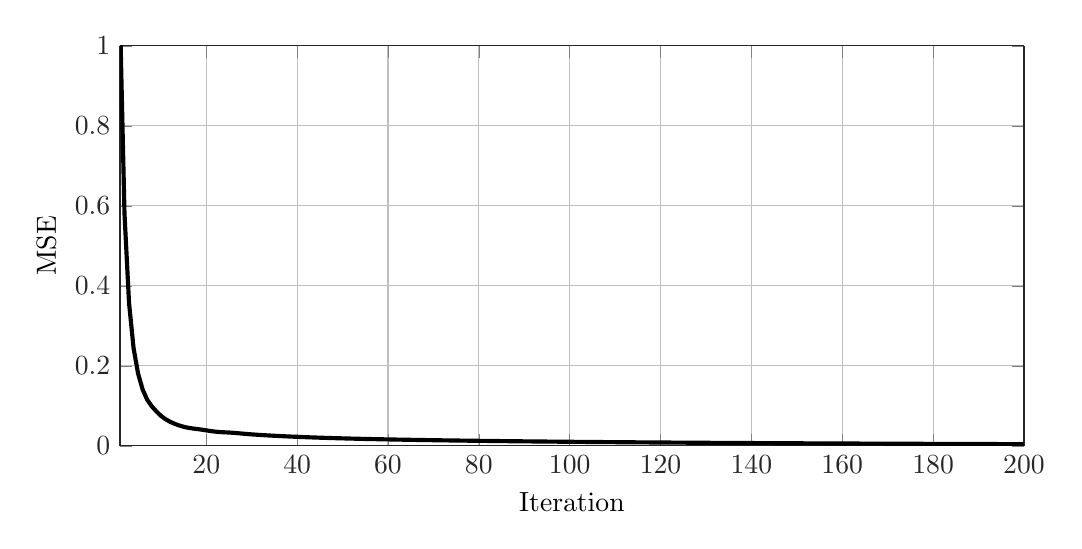
\begin{tikzpicture}
\begin{axis}[
width=4.52in,
height=2in,
scale only axis,
separate axis lines,
every outer x axis line/.append style={white!15!black},
every x tick label/.append style={font=\color{white!15!black}},
xmin=1,
xmax=200.00,
ymin=0.00,
ymax=1,
xlabel={Iteration},
ylabel={MSE},
xmajorgrids,
ymajorgrids,
every outer y axis line/.append style={white!15!black},
every y tick label/.append style={font=\color{white!15!black}},
legend style={draw=white!15!black,fill=white,legend cell align=left}]
\addplot [color=black, solid, line width=1.5pt, forget plot]
table[row sep=crcr]{
	1 1.078 \\
	2 0.58045 \\
	3 0.35746 \\
	4 0.24404 \\
	5 0.18024 \\
	6 0.14056 \\
	7 0.11511 \\
	8 0.098904 \\
	9 0.086213 \\
	10 0.075228 \\
	11 0.066742 \\
	12 0.060321 \\
	13 0.055198 \\
	14 0.05101 \\
	15 0.047662 \\
	16 0.045144 \\
	17 0.043363 \\
	18 0.041946 \\
	19 0.040394 \\
	20 0.038612 \\
	21 0.036864 \\
	22 0.035406 \\
	23 0.034381 \\
	24 0.033751 \\
	25 0.033222 \\
	26 0.032478 \\
	27 0.031502 \\
	28 0.03046 \\
	29 0.029475 \\
	30 0.028584 \\
	31 0.02778 \\
	32 0.027045 \\
	33 0.026361 \\
	34 0.025717 \\
	35 0.025105 \\
	36 0.024522 \\
	37 0.023964 \\
	38 0.023432 \\
	39 0.022924 \\
	40 0.022439 \\
	41 0.021976 \\
	42 0.021534 \\
	43 0.021112 \\
	44 0.020708 \\
	45 0.020323 \\
	46 0.019953 \\
	47 0.019599 \\
	48 0.019259 \\
	49 0.018933 \\
	50 0.018619 \\
	51 0.018316 \\
	52 0.018025 \\
	53 0.017743 \\
	54 0.017471 \\
	55 0.017208 \\
	56 0.016954 \\
	57 0.016707 \\
	58 0.016468 \\
	59 0.016235 \\
	60 0.01601 \\
	61 0.01579 \\
	62 0.015577 \\
	63 0.015368 \\
	64 0.015166 \\
	65 0.014968 \\
	66 0.014775 \\
	67 0.014587 \\
	68 0.014403 \\
	69 0.014223 \\
	70 0.014048 \\
	71 0.013876 \\
	72 0.013708 \\
	73 0.013543 \\
	74 0.013382 \\
	75 0.013223 \\
	76 0.013069 \\
	77 0.012917 \\
	78 0.012768 \\
	79 0.012621 \\
	80 0.012478 \\
	81 0.012337 \\
	82 0.012199 \\
	83 0.012063 \\
	84 0.011929 \\
	85 0.011798 \\
	86 0.011669 \\
	87 0.011542 \\
	88 0.011418 \\
	89 0.011295 \\
	90 0.011174 \\
	91 0.011056 \\
	92 0.010939 \\
	93 0.010824 \\
	94 0.010711 \\
	95 0.010599 \\
	96 0.010489 \\
	97 0.010381 \\
	98 0.010275 \\
	99 0.01017 \\
	100 0.010066 \\
	101 0.0099644 \\
	102 0.009864 \\
	103 0.009765 \\
	104 0.0096674 \\
	105 0.0095711 \\
	106 0.0094762 \\
	107 0.0093827 \\
	108 0.0092903 \\
	109 0.0091993 \\
	110 0.0091095 \\
	111 0.0090208 \\
	112 0.0089334 \\
	113 0.0088471 \\
	114 0.008762 \\
	115 0.0086779 \\
	116 0.008595 \\
	117 0.0085131 \\
	118 0.0084322 \\
	119 0.0083524 \\
	120 0.0082736 \\
	121 0.0081958 \\
	122 0.0081189 \\
	123 0.008043 \\
	124 0.0079681 \\
	125 0.007894 \\
	126 0.0078209 \\
	127 0.0077486 \\
	128 0.0076773 \\
	129 0.0076067 \\
	130 0.0075371 \\
	131 0.0074682 \\
	132 0.0074002 \\
	133 0.0073329 \\
	134 0.0072665 \\
	135 0.0072008 \\
	136 0.0071358 \\
	137 0.0070717 \\
	138 0.0070082 \\
	139 0.0069455 \\
	140 0.0068835 \\
	141 0.0068222 \\
	142 0.0067616 \\
	143 0.0067017 \\
	144 0.0066424 \\
	145 0.0065838 \\
	146 0.0065259 \\
	147 0.0064686 \\
	148 0.0064119 \\
	149 0.0063558 \\
	150 0.0063004 \\
	151 0.0062455 \\
	152 0.0061913 \\
	153 0.0061376 \\
	154 0.0060845 \\
	155 0.006032 \\
	156 0.00598 \\
	157 0.0059286 \\
	158 0.0058777 \\
	159 0.0058274 \\
	160 0.0057776 \\
	161 0.0057283 \\
	162 0.0056795 \\
	163 0.0056313 \\
	164 0.0055835 \\
	165 0.0055362 \\
	166 0.0054894 \\
	167 0.0054431 \\
	168 0.0053973 \\
	169 0.0053519 \\
	170 0.005307 \\
	171 0.0052626 \\
	172 0.0052186 \\
	173 0.005175 \\
	174 0.0051319 \\
	175 0.0050892 \\
	176 0.005047 \\
	177 0.0050051 \\
	178 0.0049637 \\
	179 0.0049227 \\
	180 0.0048821 \\
	181 0.0048419 \\
	182 0.0048021 \\
	183 0.0047626 \\
	184 0.0047236 \\
	185 0.0046849 \\
	186 0.0046467 \\
	187 0.0046087 \\
	188 0.0045712 \\
	189 0.004534 \\
	190 0.0044972 \\
	191 0.0044607 \\
	192 0.0044246 \\
	193 0.0043888 \\
	194 0.0043534 \\
	195 0.0043183 \\
	196 0.0042835 \\
	197 0.0042491 \\
	198 0.004215 \\
	199 0.0041812 \\
	200 0.0041477 \\
};

\end{axis}
\end{tikzpicture}}
\end{center}
\end{frame}

%16
\begin{frame}{An example of layered neural network}
\begin{center}
	\resizebox{\textwidth}{!}{\def\layersep{1.3cm}
\def\outsep{0.5cm}
\def\dy{0.7}

\begin{tikzpicture}[->, shorten >= 0pt, draw=black!50, node distance=\layersep,font=\fontsize{8}{8}\selectfont]
    \tikzstyle{node}=[circle,fill=black,minimum size=3pt,inner sep=0pt]
    \tikzstyle{nothing}=[draw=none,minimum size=0pt,inner sep=0pt]
    \tikzstyle{neuron}=[draw=black,circle,fill=none,minimum size=12pt,inner sep=0pt]
    \tikzstyle{HLMS neuron}=[neuron, double, double distance=2pt]

	%%%% Layer 1
    \foreach \name / \y in {1,...,5} {
    % This is the same as writing \foreach \name / \y in {1/1,2/2,3/3,4/4}
        \node[node] (I1-\name) at (0,-\dy*\y) {}; % Draw the input layer nodes
        \node[HLMS neuron] (H1-\name) at (\layersep,-\dy*\y cm) {}; % Draw the hidden layer nodes
        \node[node] (O1-\name) at (\layersep+\outsep,-\dy*\y cm) {}; % Draw the output layer node     
        \draw[->,shorten >=0cm,shorten <=0.05cm] (H1-\name) -- (O1-\name);
     }   	
    % Connect every node in the input layer with every node in the
    % hidden layer.
    \foreach \source in {1,...,5}
        \foreach \dest in {1,...,5}
            \draw[->,shorten >=0.05cm,shorten <=0cm] (I1-\source) -> (H1-\dest);

	%%%% Layer 2
    \foreach \name / \y in {1,...,5} {
    % This is the same as writing \foreach \name / \y in {1/1,2/2,3/3,4/4}
        \node[HLMS neuron] (H2-\name) at (2*\layersep+\outsep,-\dy*\y cm) {}; % Draw the hidden layer nodes
        \node[node] (O2-\name) at (2*\layersep+2*\outsep,-\dy*\y cm) {}; % Draw the output layer node
        \draw[->,shorten >=0cm,shorten <=0.05cm] (H2-\name) -- (O2-\name);
     }   	
    % Connect every node in the input layer with every node in the
    % hidden layer.
    \foreach \source in {1,...,5}
        \foreach \dest in {1,...,5}
            \draw[->,shorten >=0.05cm,shorten <=0cm] (O1-\source) edge (H2-\dest);
    
    %%%% Layer 3
    \foreach \name / \y in {1,...,5} {
    % This is the same as writing \foreach \name / \y in {1/1,2/2,3/3,4/4}
        \node[HLMS neuron] (H3-\name) at (3*\layersep+2*\outsep,-\dy*\y cm) {}; % Draw the hidden layer nodes
        \node[node] (O3-\name) at (3*\layersep+3*\outsep,-\dy*\y cm) {}; % Draw the output layer node
        \draw[->,shorten >=0cm,shorten <=0.05cm] (H3-\name) -- (O3-\name);
     }   	
    % Connect every node in the input layer with every node in the
    % hidden layer.
    \foreach \source in {1,...,5}
        \foreach \dest in {1,...,5}
            \draw[->,shorten >=0.05cm,shorten <=0cm] (O2-\source) edge (H3-\dest);
        
    %%%% Layer 4
    \foreach \name / \y in {1,...,5} {
    % This is the same as writing \foreach \name / \y in {1/1,2/2,3/3,4/4}
        \node[neuron] (H4-\name) at (4*\layersep+3*\outsep,-\dy*\y cm) {}; % Draw the hidden layer nodes
        \node[nothing] (O4-\name) at (4*\layersep+4*\outsep,-\dy*\y cm) {}; % Draw the output layer node
        \path (H4-\name) edge (O4-\name);
     }   	
    % Connect every node in the input layer with every node in the
    % hidden layer.
    \foreach \source in {1,...,5}
        \foreach \dest in {1,...,5} 
            \draw (O3-\source) edge (H4-\dest);

	%% Text
    \node[left of=I1-3, node distance=0.8cm] (in) {Inputs};
    \node[right of=O4-3, node distance=0.8cm] (out) {Outputs};
	\draw[-,decoration={brace,mirror,raise=5pt},decorate, thick]
   (0.9, -3.75) -- node[below=10pt] {Hebbian-LMS pre-processor} (5.3, -3.75);
   \draw[-,decoration={brace,mirror,raise=5pt},decorate, thick, text width=3em, text centered]
   (6.3, -3.75) -- node[below=6pt] {Softmax output layer} (7.1, -3.75);
\end{tikzpicture}}
\end{center}
\end{frame}

\begin{frame}{First layer: hyperplane separation of input pattern space}
\begin{center}
	\begin{figure}[t!]
		\centering
		\begin{subfigure}[h!]{0.5\textwidth}
			\resizebox{0.75\linewidth}{!}{\input{figs/clusters-a.tex}}\caption{}
		\end{subfigure}%
		~ 
		\begin{subfigure}[h!]{0.5\textwidth}
			\resizebox{0.75\linewidth}{!}{\input{figs/clusters-b.tex}}\caption{}
		\end{subfigure}
		
		\begin{subfigure}[h!]{0.5\textwidth}
			\resizebox{0.75\linewidth}{!}{\def\Ax{-8}
\def\Ay{15}
\def\Bx{3}
\def\By{-15}

\begin{tikzpicture} 
\begin{axis}[
axis lines*=middle,
enlargelimits = true,
xmax=20,
xmin=-20,
ymin=-20,
ymax=20,
xtick=\empty,
ytick=\empty,
  ]
  \pgfplotsinvokeforeach{1,...,100}{
  \addplot[only marks, blue, fill=white] coordinates {({\Ax+invgauss(rnd, rnd)},{\Ay+invgauss(rnd, rnd)})};
  \addplot[only marks, red, fill=white] coordinates {({\Bx+invgauss(rnd, rnd)},{\By+invgauss(rnd, rnd)})};
  }

\addplot[mark=*, only marks, black, mark size =3pt] coordinates {(\Ax,\Ay)};
\addplot[mark=*, only marks, black, mark size =3pt] coordinates {(\Bx,\By)};
  
\node at (axis cs:\Ax-6,\Ay) [anchor=east] {\Large A};  
\node at (axis cs:\Bx+6,\By) [anchor=west] {\Large B};  

\addplot[black, line width = 1pt, domain=-50:50, samples=2] {15+0.4*x};
\node at (axis cs:14, 20) [anchor=south] {\Large $+$};
\node at (axis cs:15, 16) [anchor=south] {\Large $-$};
\end{axis}
\end{tikzpicture}
}\caption{}
		\end{subfigure}%
		~ 
		\begin{subfigure}[h!]{0.5\textwidth}
			\resizebox{0.75\linewidth}{!}{\input{figs/clusters-d.tex}}\caption{}
		\end{subfigure}   
	\end{figure}
\end{center}
\end{frame}

\begin{frame}{Statistical pattern classification}
\begin{equation*}
	\rho = \frac{\text{standard deviation of patterns in each cluster}}{\text{average distance between centroids}} \tag{difficulty metric}
\end{equation*}
\begin{center}
	\resizebox{0.75\textwidth}{!}{\pgfmathsetseed{11}%
\pgfmathsetmacro\Ax{invgauss(rnd, rnd)}
\pgfmathsetmacro\Ay{invgauss(rnd, rnd)}
\pgfmathsetmacro\Bx{invgauss(rnd, rnd)}
\pgfmathsetmacro\By{invgauss(rnd, rnd)}
\pgfmathsetmacro\Cx{invgauss(rnd, rnd)}
\pgfmathsetmacro\Cy{invgauss(rnd, rnd)}
\pgfmathsetmacro\Dx{invgauss(rnd, rnd)}
\pgfmathsetmacro\Dy{invgauss(rnd, rnd)}

\def\r{0.15}

\begin{tikzpicture} 
\begin{axis}[
axis lines*=middle,
enlargelimits = true, clip=true,
axis equal,
xtick=\empty,
ytick=\empty,
  ]
  \draw[blue!20, fill=blue!20] (\Ax, \Ay) circle (4*\r);
  \draw[red!20, fill=red!20] (\Bx, \By) circle (4*\r);
  \draw[green2!20, fill=green2!20] (\Cx, \Cy) circle (4*\r);
  \draw[orange2!20, fill=orange2!20] (\Dx, \Dy) circle (4*\r);
  \pgfplotsinvokeforeach{1,...,100}{
  \addplot[only marks, blue, fill=white] coordinates {({\Ax+\r*invgauss(rnd, rnd)},{\Ay+\r*invgauss(rnd, rnd)})};
  \addplot[only marks, red, fill=white] coordinates {({\Bx+\r*invgauss(rnd, rnd)},{\By+\r*invgauss(rnd, rnd)})};
  \addplot[only marks, green2, fill=white] coordinates {({\Cx+\r*invgauss(rnd, rnd)},{\Cy+\r*invgauss(rnd, rnd)})};
  \addplot[only marks, orange2, fill=white] coordinates {({\Dx+\r*invgauss(rnd, rnd)},{\Dy+\r*invgauss(rnd, rnd)})};
  }

\addplot[mark=*, only marks, black, mark size =3pt] coordinates {(\Ax,\Ay)};
\addplot[mark=*, only marks, black, mark size =3pt] coordinates {(\Bx,\By)};
\addplot[mark=*, only marks, black, mark size =3pt] coordinates {(\Cx,\Cy)};
\addplot[mark=*, only marks, black, mark size =3pt] coordinates {(\Dx,\Dy)};
  
\end{axis}
\end{tikzpicture}
}
\end{center}
Example of 4 clusters in 2-D
\end{frame}

\begin{frame}{LMS capacity}
\begin{block}{Single neuron}
	\begin{equation*}
	\text{Capacity} = \text{number of weights}
	\end{equation*}
\end{block}

\begin{block}{Layered network}
	\begin{equation*}
	\text{Capacity} = \text{number of weights of output-layer neuron}
	\end{equation*}
\end{block}

\end{frame}

\begin{frame}{Good practice for hyper-parameter selection}
\begin{itemize}
\item The input patterns should be normalized to have zero mean and unit variance

\item The adaptation ratio of each neuron should be
\begin{equation*}
	\mu = \frac{0.1}{\text{number of the neuron's weights}}
\end{equation*} 
\item The Hebbian-LMS parameter $\gamma$ should be between 0.3 to 0.5

\item The initial weights of each neuron may be Gaussian distributed with zero mean and variance 
\begin{equation*}
	\sigma_w^2 = \frac{\gamma^2}{4}
\end{equation*} 
\end{itemize}
\end{frame}

\begin{frame}{Statistical pattern classification}

Classification error for 100 clusters in 50-dimensional space

Neural network had 3 hidden layers with 150 neurons/hidden layer.

\begin{center}
	\resizebox{0.7\textwidth}{!}{\begin{tikzpicture}
\begin{axis}[
width=4.52in,
height=3.56in,
%scale only axis,
separate axis lines,
every outer x axis line/.append style={white!15!black},
every x tick label/.append style={font=\color{white!15!black}},
xmin=0.00,
xmax=50.00,
ymin=0.00,
ymax=40.00,
xlabel={\Large Training cycles},
ylabel={\Large Error rate ($\%$)},
xmajorgrids,
ymajorgrids,
every outer y axis line/.append style={white!15!black},
every y tick label/.append style={font=\color{white!15!black}},
legend style={draw=white!15!black,fill=white,legend cell align=left, at={(0.667262,0.748413)},anchor=south west}]

\addplot [smooth, color=blue2, dashed, line width=2pt, forget plot] table[x index=0,y index=5] {figs/hlms_rho.dat}; %\addlegendentry{$\rho = 5.0\%$};
\addplot [smooth, color=blue2, solid, line width=2pt] table[x index=0,y index=6] {figs/hlms_rho.dat}; \addlegendentry{$\rho = 5.0\%$};

\addplot [smooth, color=red, dashed, line width=2pt, forget plot] table[x index=0,y index=3] {figs/hlms_rho.dat}; %\addlegendentry{$\rho = 5.0\%$};
\addplot [smooth, color=red, solid, line width=2pt] table[x index=0,y index=4] {figs/hlms_rho.dat}; \addlegendentry{$\rho = 7.5\%$};

\addplot [smooth, color=green2, dashed, line width=2pt, forget plot] table[x index=0,y index=1] {figs/hlms_rho.dat} node[pos=0.85, black, pin={[pin edge={black, thick}]20:{\Large \color{black}  Test set}}, inner sep=0pt] {}; %\addlegendentry{$\rho = 5.0\%$};
\addplot [smooth, color=green2, solid, line width=2pt] table[x index=0,y index=2] {figs/hlms_rho.dat} node[pos=0.85, black, pin={[pin edge={black, thick}]20:{\Large \color{black} Training set}}, inner sep=0pt] {}; \addlegendentry{$\rho = 10.0\%$};

\end{axis}
\end{tikzpicture}}
\end{center}

Training set had 20 samples/cluster, while test set had 80 samples/cluster.
% (\sampleline{}) error on the training set
% (\sampleline{dashed}) error on the test set
\end{frame}


\begin{frame}{A biological form of Hebbian-LMS}
\begin{center}
	\includegraphics[page=12,width=\textwidth, trim={0.5cm 2.5cm 0.5cm 1.25cm}, clip]{figures.pdf}
\end{center}
\end{frame}

\begin{frame}{Hidden layers: clustering example}
\begin{center}
	\includegraphics[page=21,width=\textwidth, trim={0.2cm 3.75cm 0.2cm 1.5cm}, clip]{figures.pdf}
\end{center}
\large 50-dimensional input vectors plotted among the first two principal components.
\end{frame}

\begin{frame}{Hidden layers: clustering example}
\begin{center}
\includegraphics[page=22,width=\textwidth, trim={0.2cm 3.75cm 0.2cm 1.5cm}, clip]{figures.pdf}
\end{center}
\large Histogram of responses of a selected neuron in the output layer of a
three-layer Hebbian-LMS network.
\end{frame}

\begin{frame}{Hidden layers: clustering example}
\begin{center}
\includegraphics[page=23,width=\textwidth, trim={0.2cm 3.75cm 0.2cm 1.5cm}, clip]{figures.pdf}
\end{center}
\large Histogram of responses of a selected neuron in the output layer of a three-layer Hebbian-LMS network.
\end{frame}

\begin{frame}{A synapse corresponding to a variable weight}
\begin{center}
	\includegraphics[page=25,width=\textwidth, trim={0.5cm 3.5cm 0.5cm 1.5cm}, clip]{figures.pdf}
\end{center}
\end{frame}

\begin{frame}{Neurons, dendrites, and a synapse}
\begin{center}
	\includegraphics[page=26,width=\textwidth, trim={0.2cm 2.25cm 0.5cm 1.5cm}, clip]{figures.pdf}
\end{center}
\end{frame}

\begin{frame}{Postulates of synaptic plasticity}
\begin{itemize}
	\setlength\itemsep{1em}
	\item When the pre-synaptic neuron is not firing, there will be no neurotransmitter in the gap and there will be no weight change. This applies to both excitatory and inhibitory synapses.
	\item When the pre-synaptic neuron is firing, and the post-synaptic neuron is also firing, there will be neurotransmitter in the gap and the post-synaptic membrane voltage will be positive since the (SUM) is positive, and the number of neuroreceptors will gradually increase, thus increasing the weight. This applies to excitatory synapses. This is Hebb's rule.
	\item When the pre-synaptic neuron is firing, and the post-synaptic neuron is not firing, there will be neurotransmitter in the gap and the post-synaptic membrane voltage will be negative since the (SUM) is negative and its number of neuroreceptors will gradually decrease, thus decreasing the weight. This applies to excitatory synapses.
	\item The opposite of these rules apply to inhibitory synapses.
\end{itemize}
\end{frame}



\end{document}
